\documentclass[a4paper,12pt]{article}
\usepackage[utf8]{inputenc}
\usepackage[spanish]{babel}
\usepackage{amsmath}
\usepackage{graphicx}
\usepackage{tocbibind}
\usepackage{hyperref}
% \usepackage{cite}

% \title{Linus Torvalds y el desarrollo de Linux}
% \author{José Antonio Concepción Alvarez\\  José Miguel Zayas Pérez \\ Grupo: 411 y 412}
% \date{\today}

\begin{document}

% Portada
% \maketitle

\begin{titlepage}
    \centering
    
    % Incluir la imagen
    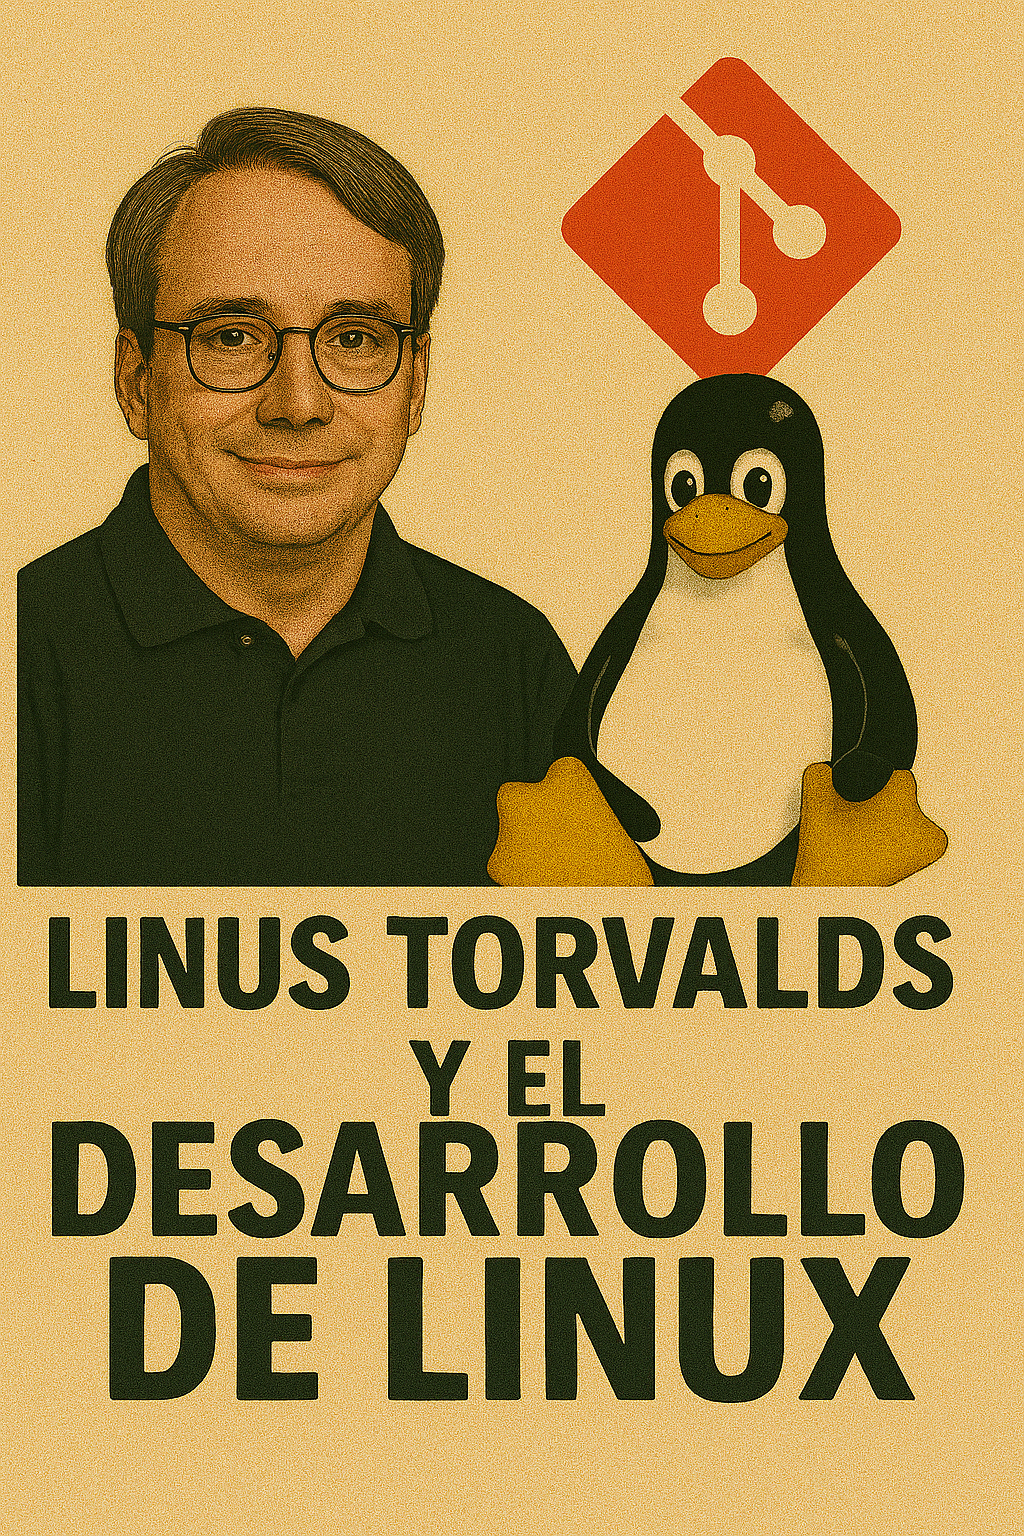
\includegraphics[width=1.0\textwidth]{images/front.png} % Cambia la ruta a la ubicación de tu imagen
    
    \vspace{1cm}
    \newpage
    
    % Título
    {\Huge \textbf{Linus Torvalds y el desarrollo de Linux}}\\
    \vspace{0.5cm}
    
    % Autores
    {\Large José Antonio Concepción Alvarez \\  José Miguel Zayas Pérez \\ Grupo: 411 y 412}
    
    % \vfill
    
    % Fecha
    % {\large \today}
   \thispagestyle{empty} 
\end{titlepage}

\begin{centering}
    \vspace{2cm}
    \textbf{Resumen}\\
    Este ensayo explora la vida y las contribuciones de Linus Torvalds, el
    creador del núcleo Linux y Git, y su impacto en la historia de la
    computación. Se presenta un análisis de su relevancia en el desarrollo del
    software libre y de código abierto, destacando cómo su trabajo ha
    transformado el desarrollo colaborativo en la industria del software. A
    través de un examen de los antecedentes históricos, el nacimiento y
    evolución de Linux, y su influencia en la infraestructura de internet y
    dispositivos móviles, se argumenta que la influencia de Torvalds va más allá
    de la creación de software, abarcando un legado de colaboración y
    transparencia en el desarrollo tecnológico. Finalmente, se reflexiona sobre
    su impacto en el futuro de la tecnología y la filosofía del código abierto.
\end{centering}
\newpage

% Índice
\tableofcontents
\newpage

% Sección 1
\section{Introducción} 

En la vasta cronología de la historia de la computación, pocos nombres han
dejado una huella tan profunda y duradera como el de Linus Torvalds. Reconocido
mundialmente como el creador del núcleo del sistema operativo Linux y del
sistema de control de versiones distribuido Git, Torvalds ha sido una figura
clave en la evolución del software moderno. Su obra no solo ha influido en la
infraestructura tecnológica global, sino que también ha catalizado una
transformación en la manera en que el software es desarrollado, compartido y
perfeccionado.

El núcleo Linux, iniciado como un proyecto personal en 1991, se ha convertido en
el corazón de millones de sistemas, desde servidores y supercomputadoras hasta
dispositivos móviles. A su vez, Git, concebido inicialmente para gestionar el
desarrollo del propio kernel de Linux, se ha posicionado como la herramienta
estándar para el control de versiones en proyectos de cualquier escala. Sin
embargo, más allá de estos hitos técnicos, la relevancia de Torvalds se extiende
a un plano más amplio: su trabajo ha redefinido las dinámicas del desarrollo
colaborativo, sentando las bases del movimiento de código abierto y fomentando
una cultura de cooperación, transparencia y meritocracia técnica.

Este trabajo abordará la influencia de Linus Torvalds en el desarrollo de
software, el crecimiento de la comunidad de Open Source, la colaboración a gran
escala y la consolidación de un modelo de innovación abierto que ha transformado
profundamente la industria tecnológica y la cultura digital contemporánea.  
\newpage

% Sección 2
\section{Antecedentes} 
- Contexto histórico de la computación antes de la
aparición de Linux.\\ 

% ¿Qué sistemas operativos dominaban el mercado antes de la llegada de Linux?

% ¿Cuál era el modelo de desarrollo de software predominante en esa época?
% ¿Qué papel tenían las universidades y los gobiernos en el desarrollo de software?
% ¿Qué limitaciones técnicas y filosóficas presentaban los sistemas propietarios
% existentes?
% ¿Cómo era la relación entre los usuarios y el software que
% utilizaban?


- El surgimiento del movimiento del software libre y de
código abierto.\\ 
- La trayectoria temprana de Linus Torvalds y su motivación
para desarrollar Linux.

% Sección 3
\section{El Nacimiento y Evolución de Linux} 
- El desarrollo inicial de Linux
como un proyecto personal.\\ 
- La transición de Linux a un proyecto colaborativo
global.\\ 
- El impacto de la Licencia Pública General de GNU (GPL) en la
expansión de Linux.\\ 
- La evolución de Linux y su adopción en servidores,
dispositivos móviles y sistemas embebidos.

% Sección 4
\section{El Impacto de Linux en la Industria de la Computación} 
- La influencia
de Linux en el desarrollo de servidores y la infraestructura de internet.\\ 
- El
papel de Linux en la revolución de los dispositivos móviles a través de
Android.\\ 
- La adopción de Linux en supercomputadoras y sistemas de alto
rendimiento.\\ 
- El impacto económico y social de Linux.

% Sección 5
\section{Linus Torvalds y el Desarrollo Colaborativo} 
- El modelo de desarrollo
de Linux y su influencia en la colaboración en línea.\\ 
- El papel de Torvalds
como líder y coordinador de la comunidad de Linux.\\ 
- El impacto de Git en la
gestión de versiones y la colaboración en proyectos de software.

% Sección 6
\section{La Filosofía del Código Abierto y su Difusión} 
- La defensa de Torvalds
del código abierto y su impacto en la industria del software.\\ 
- La influencia
de Linux en la adopción del código abierto en empresas y organizaciones.\\ 
- El
legado de Torvalds en la promoción de la transparencia y la colaboración en el
desarrollo de software.

% Sección 7
\section{Conclusiones} 
- Resumen de las contribuciones clave de Linus
Torvalds.\\ 
- Reafirmación de la tesis sobre su influencia en la computación.\\

- Reflexión sobre el legado de Torvalds y su impacto en el futuro de la
tecnología.a
\newpage

\begin{thebibliography}{9}

\bibitem{mochi_aleman_movimiento_2015}
Mochi Alemán, Prudencio Óscar, \textit{El movimiento del software libre}, Revista Mexicana de Ciencias Políticas y Sociales, vol. 45, no. 185, 2015. URL: \url{http://www.revistas.unam.mx/index.php/rmcpys/article/view/48320}.

\bibitem{stallman_free_2002}
Stallman, Richard y Stallman, Richard M., \textit{Free software, free society: selected essays}, 1st ed., Free Software Foundation, Boston, Mass, 2002. ISBN: 978-1-882114-98-6.

\bibitem{campbell-kelly_computer_1996}
Campbell-Kelly, Martin y Aspray, William, \textit{Computer: a history of the information machine}, BasicBooks, New York, 1996. ISBN: 978-0-465-02989-1.

\bibitem{torvalds_just_2002}
Torvalds, Linus y Diamond, David, \textit{Just for fun: the story of an accidental revolutionary}, 1. HarperBusiness paperback ed., Harper, New York, 2002. ISBN: 978-0-06-662073-2.

\end{thebibliography}

\end{document}

